\section{Análise Exploratória de Dados (EDA)}

A primeira etapa do projeto consistiu em realizar uma análise exploratória sobre os dados de tráfego para
compreender suas características fundamentais.
O \emph{dataset} original, após ser processado, resultou em uma série temporal de volume de tráfego agregado
por segundo. O primeiro \emph{dataset} escolhido para análise foi o \texttt{200701251400.dump.gz}, por conter
um volume maior de dados.

\begin{table}[!htb]
    \centering
    \caption{Estatísticas descritivas para a série temporal do \texttt{200701251400.dump.gz}.}
    \label{tab:eda-describe}
    ../../results/200701251400.describe.tex
\end{table}

As estatísticas descritivas na \Cref{tab:eda-describe} fornecem um resumo de alto nível da intensidade do
tráfego de rede durante o período de captura de 15 minutos. O tráfego apresenta uma média de aproximadamente
1,27 MiB/s. No entanto, o desvio padrão é relativamente alto, 124,5 KiB/s, o que representa cerca de 10\% da
média. No entanto, podemos ver que essa instabilidade não aparece na série temporal da
\Cref{fig:eda-timeseries}, o que indica que as bordas da série causam esse alto valor de desvio padrão.

\begin{figure}[!htb]
    \centering
    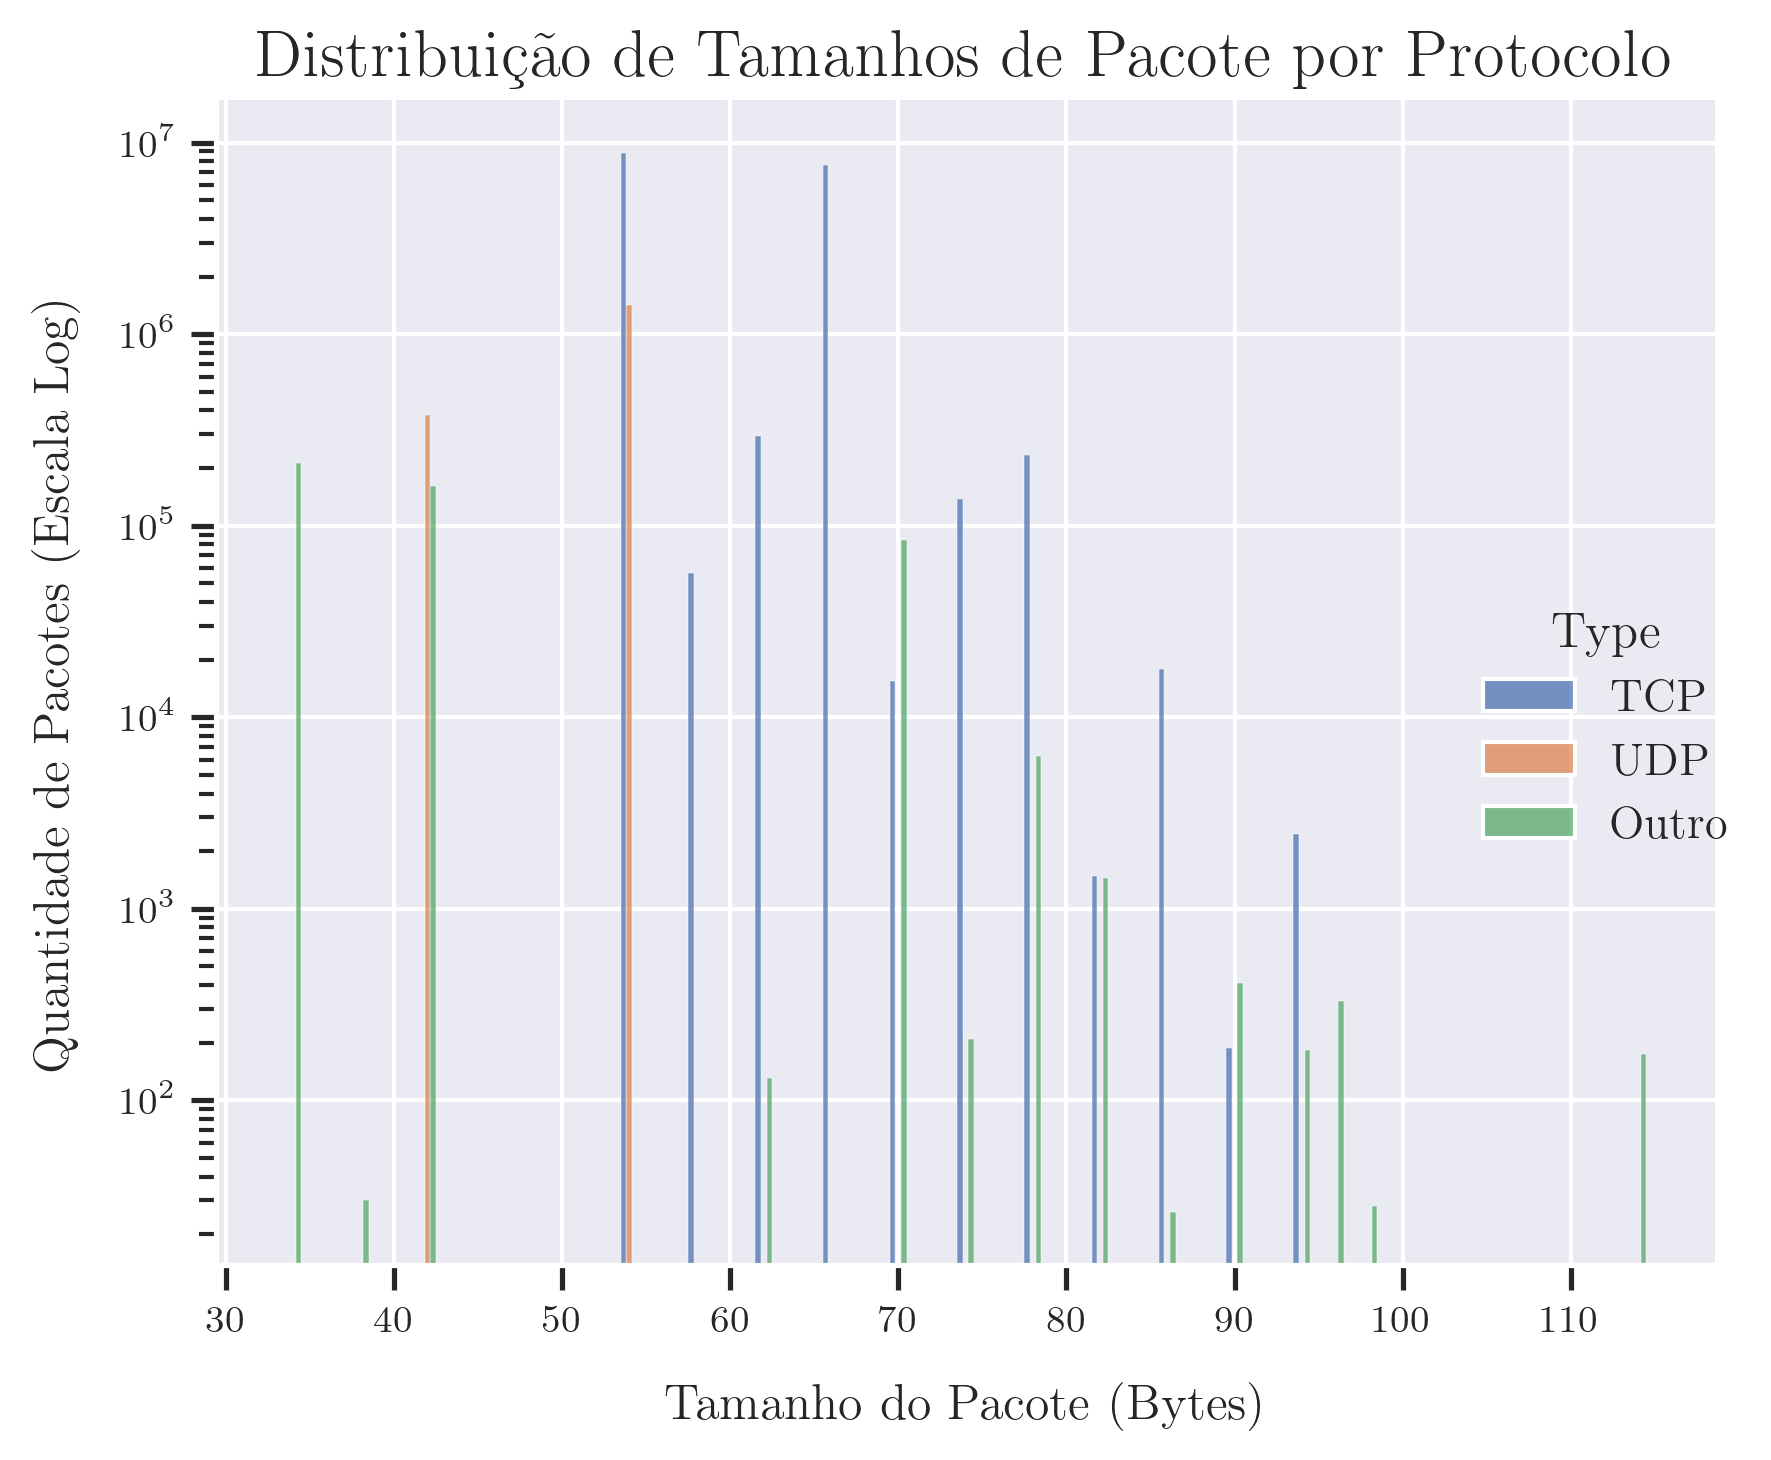
\includegraphics[width=0.95\textwidth]{resource/200701251400.protocol_dist.png}
    \caption{Distribuição de tamanhos de pacote para os protocolos TCP e UDP em
        \texttt{200701251400.dump.gz}. A frequência (eixo Y) está em
    escala logarítmica para melhor visualização.}
    \label{fig:eda-protocol-dist}
\end{figure}

\begin{figure}[!htb]
    \centering
    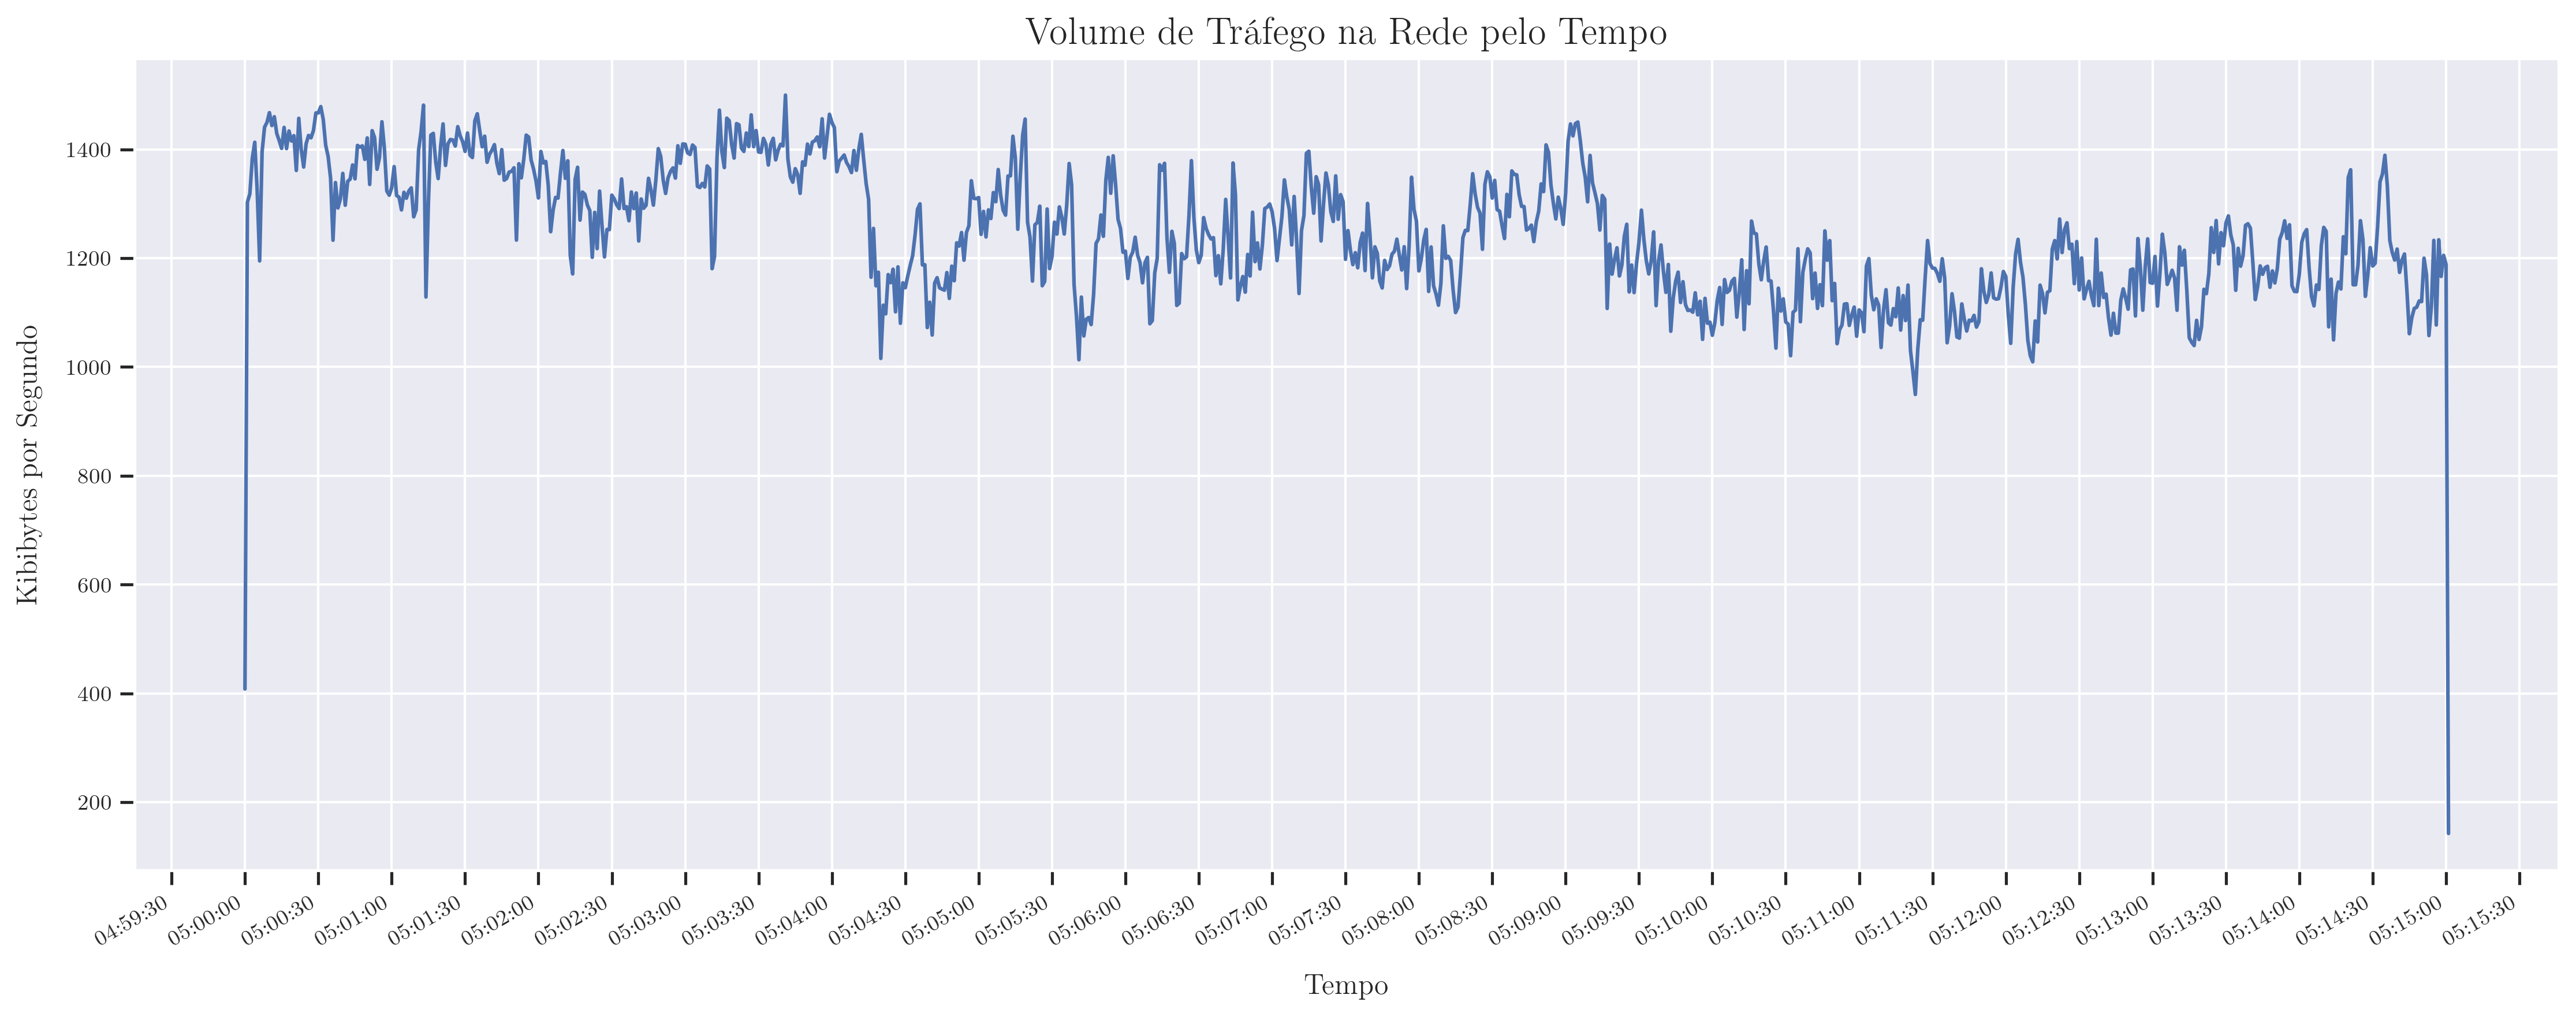
\includegraphics[width=0.95\textwidth]{resource/200701251400.time_series.png}
    \caption{Série temporal do volume de tráfego agregado por segundo.}
    \label{fig:eda-timeseries}
\end{figure}

O gráfico do tráfego agregado ao longo do tempo na \Cref{fig:eda-timeseries} oferece uma visão intuitiva do
comportamento dos dados. A série parece ter uma linha de base relativamente estável em torno de 1,2-1,4
MiB/s. Não há tendências óbvias e de longo prazo para cima ou para baixo nessa janela de 15 minutos, mas há
``regimes'' claros em que o tráfego é maior e mais volátil, seguido por períodos em que é menor e mais
estável. As quedas repentinas no início e no final são provavelmente artefatos do início e da interrupção da captura.

\begin{figure}[!htb]
    \centering
    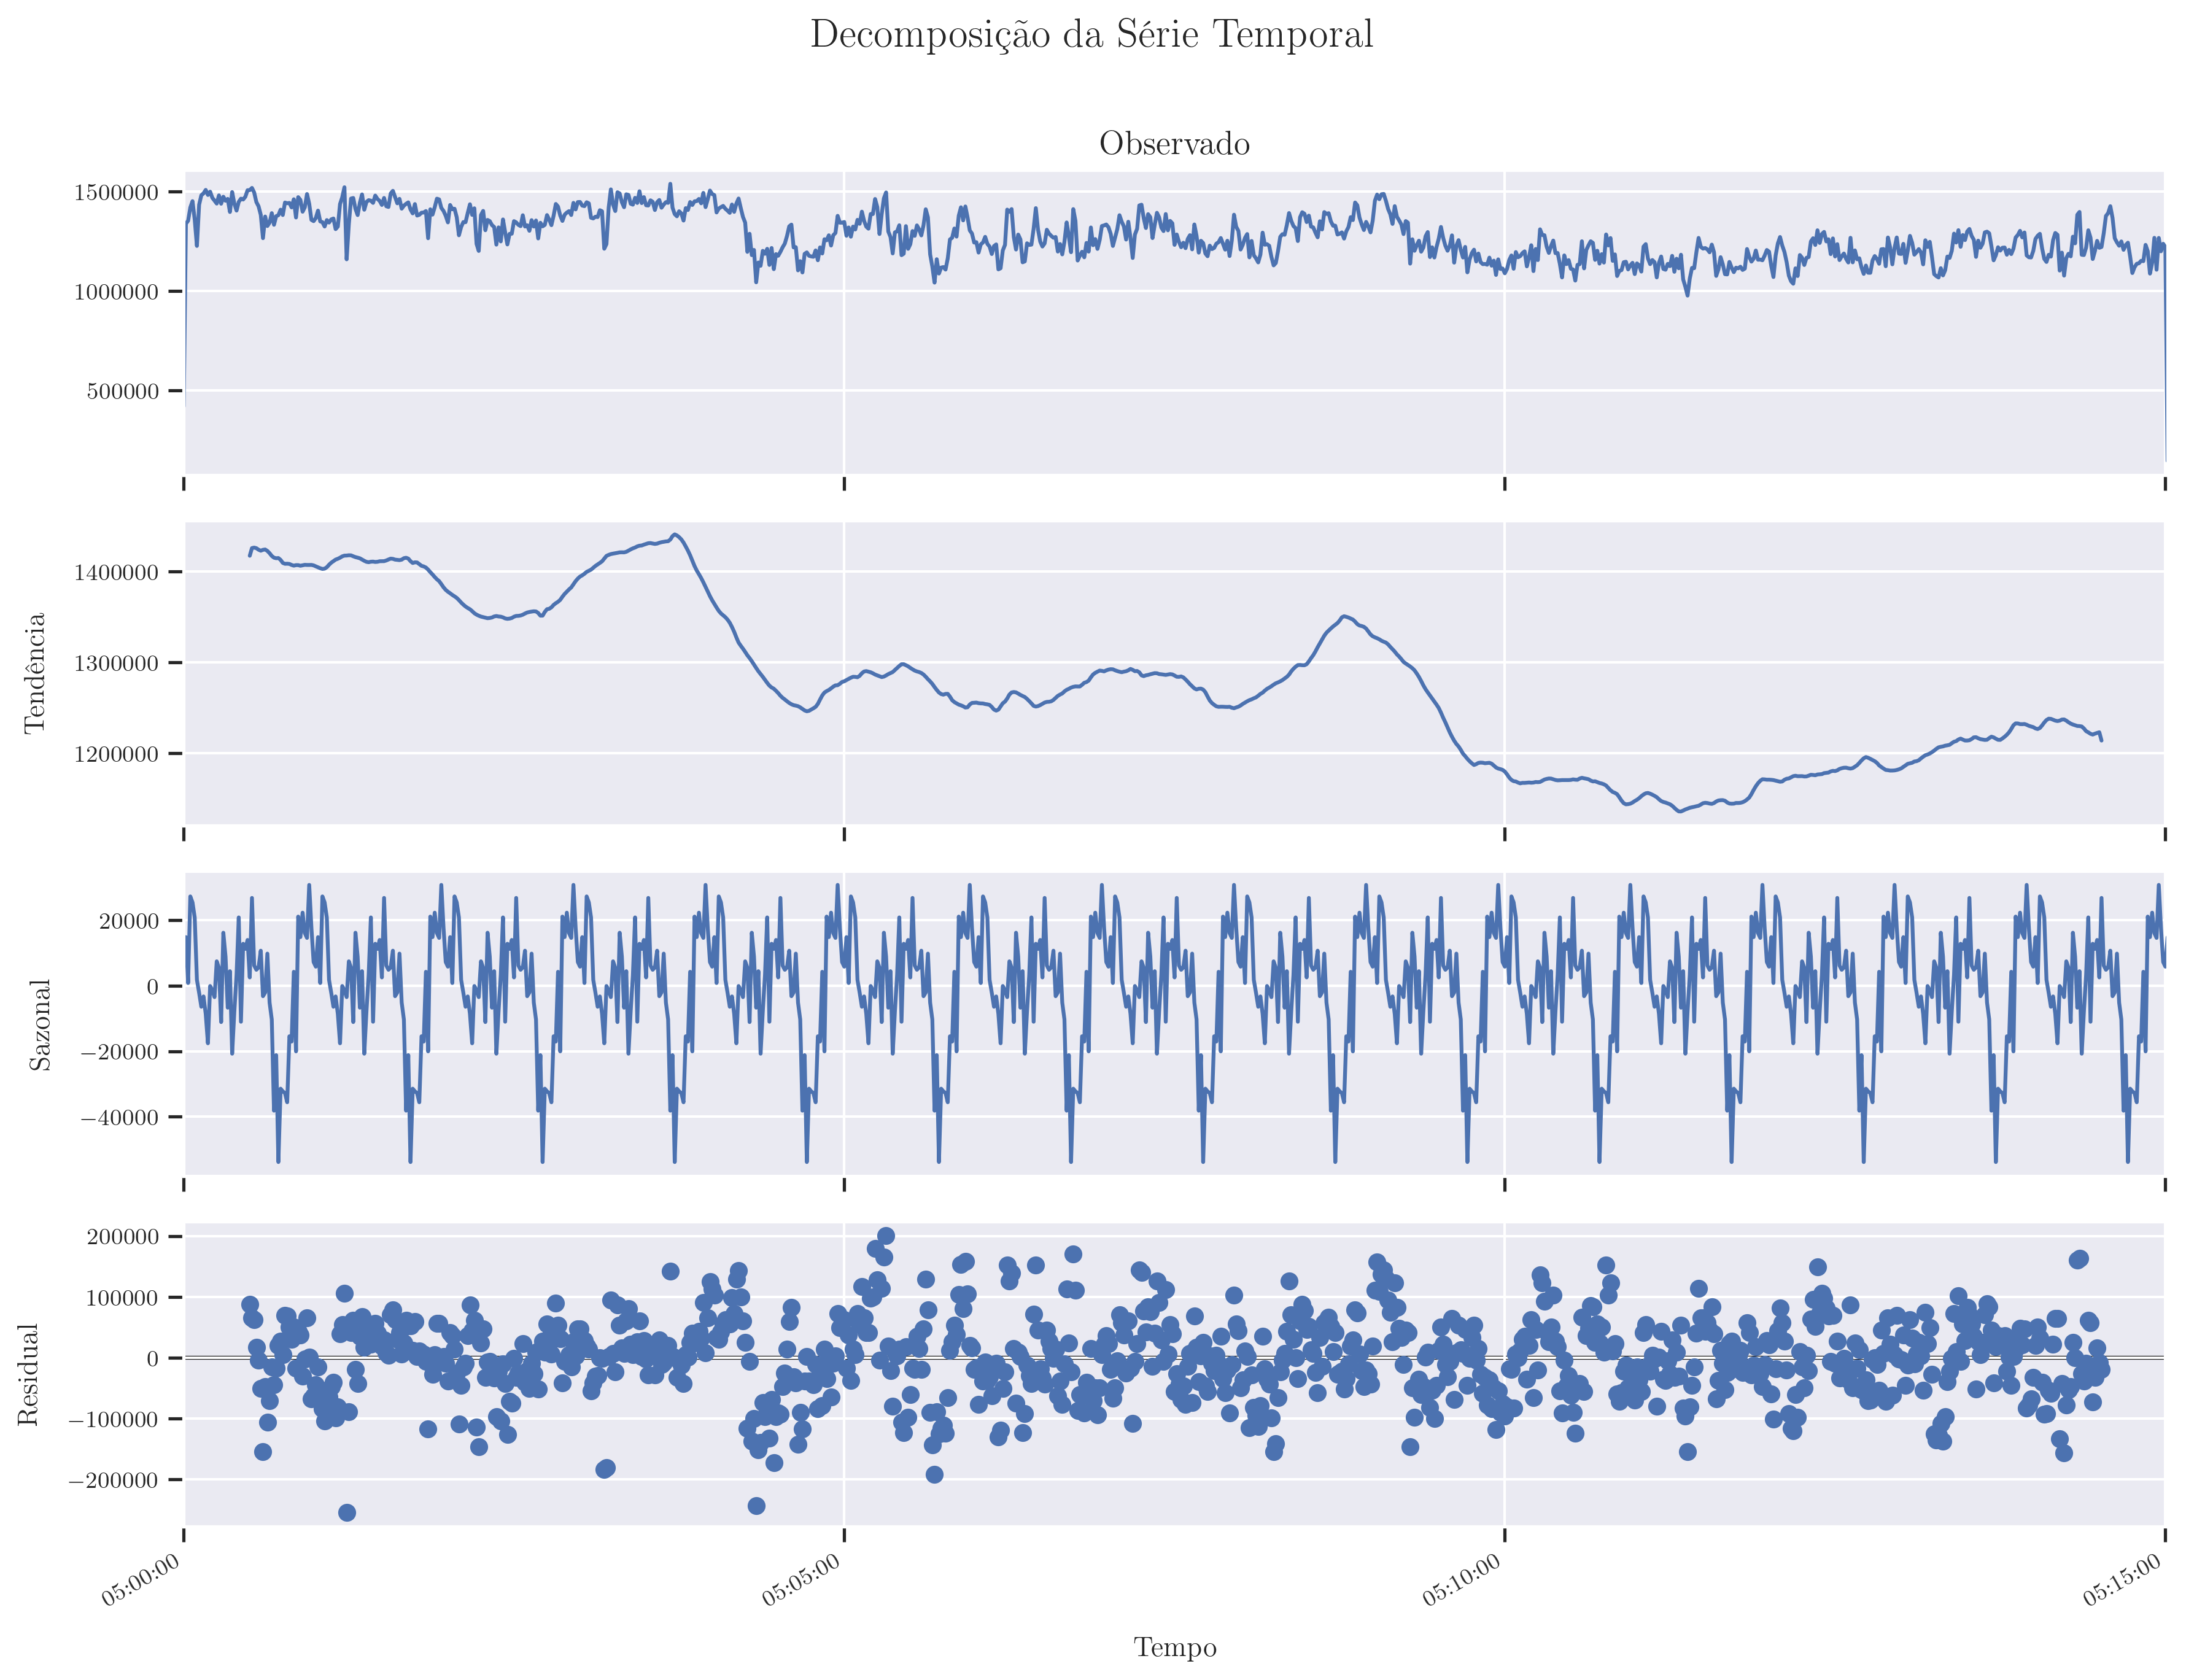
\includegraphics[width=0.8\textwidth]{resource/200701251400.decomposition.png}
    \caption{Decomposição da série temporal em tendência, sazonalidade e resíduos, com um período sazonal de
    60 segundos.}
    \label{fig:eda-decomposition}
\end{figure}

Para uma análise mais aprofundada, decompomos a série em seus componentes de tendência, sazonalidade e
resíduos, como visto na .
[... Adicione seus comentários sobre a tendência de longo prazo e os padrões periódicos (sazonais) que o
modelo precisará aprender ...]

A análise de decomposição na \Cref{fig:eda-decomposition} fornece os insights mais profundos. A componente de
tendência revela as alterações subjacentes e lentas no volume de tráfego. Podemos ver uma diminuição gradual
na carga geral de tráfego desde o início até por volta da marca de 05:08, após o que ela começa a se
recuperar ligeiramente. Isso mostra que a série não é completamente estacionária.

O componente sazonal mostra claramente um padrão forte e repetitivo com um período de 60 segundos. Isso pode
ser bem útil, pois indica um comportamento cíclico no uso da rede, talvez causado por processos automatizados
em segundo plano, ferramentas de monitoramento ou comportamentos agregados de usuários que se repetem minuto
a minuto. Por fim, o componente residual mostra o ``ruído'' ou as flutuações aleatórias deixadas após a
remoção da tendência e da sazonalidade.

\begin{figure}[!htb]
    \centering
    \includegraphics[width=0.7\textwidth]{resource/200701251400.autocorrelation.png}
    \caption{Funções de Autocorrelação (ACF) e Autocorrelação Parcial (PACF) para a série temporal.}
    \label{fig:eda-acf-pacf}
\end{figure}

Por fim, os gráficos ACF e PACF na \Cref{fig:eda-acf-pacf} fornecem uma confirmação estatística dos padrões
observados anteriormente.
O gráfico da ACF mostra um decaimento muito lento. A correlação com valores passados permanece alta mesmo
depois de alguns pontos, o que é um sinal clássico de uma não estacionariedade nos dados. Ela também confirma
que o valor do tráfego em um segundo é altamente dependente do valor do segundo anterior.

O gráfico PACF é crucial para a escolha da janela look_back. Ele mostra um pico muito grande na defasagem 1,
indicando uma forte correlação direta com o valor imediatamente anterior. Em seguida, a correlação cai
drasticamente, tornando-se estatisticamente insignificante após cerca de 10 a 12 defasagens. Isso fornece uma
forte justificativa estatística para experimentar uma janela look_back de 10, pois ela representa a memória
de curto prazo mais significativa da série.
